%\documentclass{beamer}

%%\usepackage[unicode]{hyperref}
%\title{Detekce objektů z hloubkových dat}
%\author{Lukáš Kunt}
%\institute{České vysoké učení technické v Praze}
%\date{00.00.2020}

\documentclass{beamer}
\usepackage[utf8]{inputenc}
\hypersetup{unicode = true}

\usetheme{Madrid}
\usepackage{colortbl} %use in the preamble
  
\definecolor{cvut_navy}{HTML}{0065BD}
\definecolor{cvut_blue}{HTML}{6AADE4}
\definecolor{cvut_gray}{HTML}{156570}

\setbeamercolor{section in toc}{fg=black,bg=white}
\setbeamercolor{alerted text}{fg=cvut_blue}
\setbeamercolor*{palette primary}{bg=cvut_navy,fg=gray!20!white}
\setbeamercolor*{palette secondary}{bg=cvut_blue,fg=white}
\setbeamercolor*{palette tertiary}{parent=palette primary}
\setbeamercolor*{palette quaternary}{fg=green,bg=gray!5!white}

\setbeamercolor*{sidebar}{fg=cvut_navy,bg=gray!15!white}


\setbeamercolor{titlelike}{parent=palette primary}
\setbeamercolor{frametitle}{parent=palette primary}

\setbeamercolor*{separation line}{}
\setbeamercolor*{fine separation line}{}

\setbeamertemplate{navigation symbols}{} 


\usepackage{eqnarray,amsmath}
\usepackage{amsfonts}
\usepackage{amssymb}
\usepackage{graphicx}
\usepackage{lmodern} % pro pismo tucne a zaroven kurziva
\usepackage{bm} % pro pismo tucne a zaroven kurziva
\usepackage{epstopdf}
\usepackage{changepage}
\usepackage{array,booktabs}

% definice makra pro české uvozovky:
\newcommand{\CC}{C\nolinebreak\hspace{-.05em}\raisebox{.4ex}{\tiny\bf +}\nolinebreak\hspace{-.10em}\raisebox{.4ex}{\tiny\bf +}}
\def\bq{\mbox{\kern.1ex\protect\raisebox{-1.3ex}[0pt][0pt]{''}\kern-.1ex}}
\def\eq{\mbox{\kern-.1ex``\kern.1ex}}
\def\ifundefined#1{\expandafter\ifx\csname#1\endcsname\relax }%
\ifundefined{uv}%
        \gdef\uv#1{\bq #1\eq}
\fi
% konec .... použití makra pro psaní český uvozovek: \uv{text uvnitř uvozovek}

%====================================================
%========== DEFINITION OF AUTHORS ETC...=============
%====================================================
%\author[Lukáš Kunt]{Lukáš Kunt}
\author[Lukáš Kunt]{{\large Lukáš Kunt} {\small \texorpdfstring{\vspace{5mm} \newline Vedoucí práce: RNDr. Petr Štěpán, Ph.D. }{}}}
\institute[ČVUT]{České vysoké učení technické v Praze \\ Fakulta elektrotechnická}
\title[Detekce objektů z hloubkové kamery]{Detekce objektů z hloubkové kamery}
%\subtitle{Subtitle}
\date[00.00.2020]{00.00.2020}


\begin{document}

%\placelogotrue
\frame{\titlepage
    \begin{center}

\includegraphics[height=1.3cm]{symbol_cvut_plna_samostatna_verze.pdf}
\end{center}
}

\logo{
\includegraphics[height=1cm]{symbol_cvut_plna_samostatna_verze.pdf}}
%\placelogotrue

\begin{frame}
    \frametitle{Motivace a cíle práce}
    \textbf{Motivace práce}: Detekce cihel v soutěži Mohamed Bin Zayed International Robotics Chalenge (MBZIRC). \\
    \textbf{Cíle práce}:
    \begin{itemize}
        \item Seznámení se s metodami detekce z hloubkových dat
        \item Navržení algoritmu pro detekci objektů (cihel) z hloubkových dat
        \item Implementování programu  v jazyce \CC
        \item Ověření programu na datech z kamery 
    \end{itemize}
    \begin{figure}
        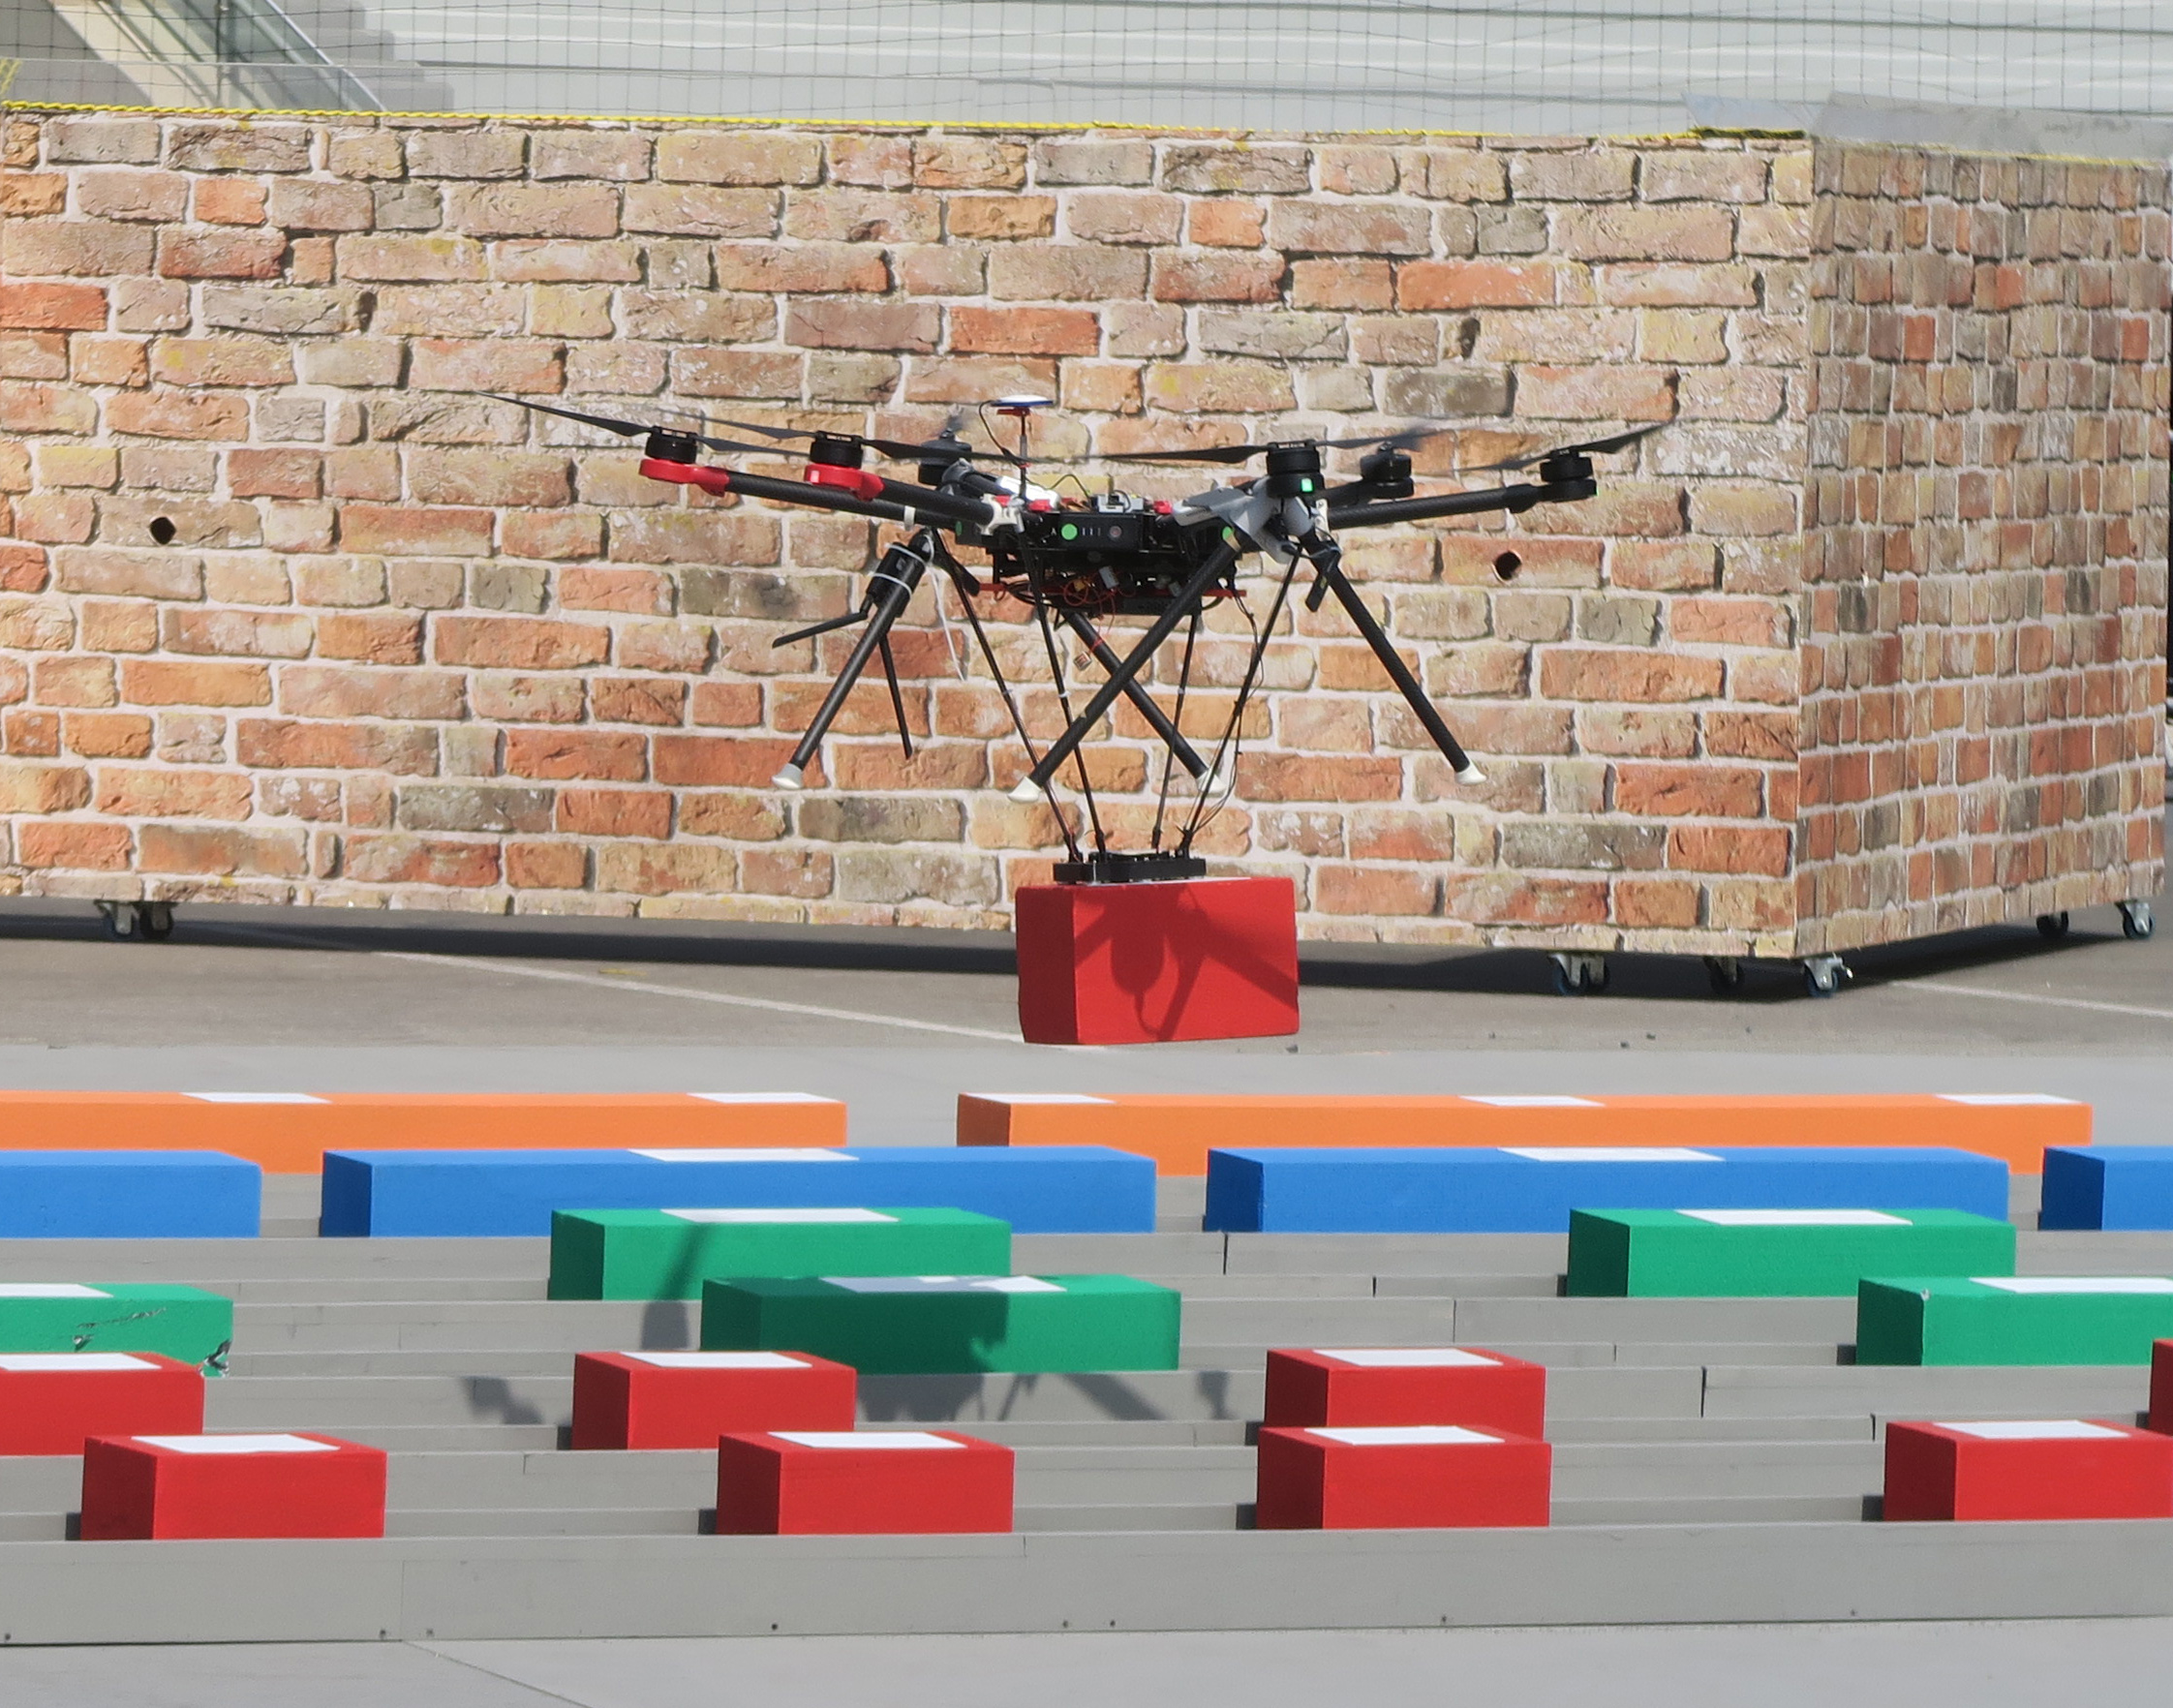
\includegraphics[width = 0.44\linewidth]{mbzirc.jpg}
    \end{figure}
\end{frame}
%\placelogofalse
\begin{frame}
    %\frametitle{Intel\textregistered{} RealSense$^{TM}$ D435}
    \frametitle{Intel RealSense$^{TM}$ D435}
   \begin{minipage}{.55\textwidth}
    \begin{itemize}
        \item RGB modul
        \item Dvojice infračervených kamer
        \item Infračervený projektor
        \item Dedikovaný procesor pro zpracování dat z infračervených kamer 
    \end{itemize}
    \end{minipage}
    \begin{minipage}{.43\textwidth}
      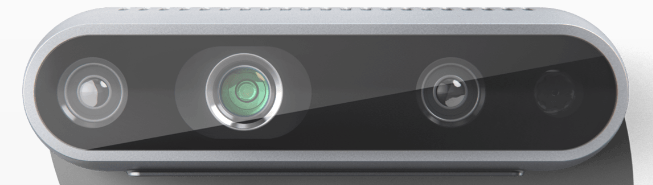
\includegraphics[width = \textwidth]{realsense_kamera.png}
    \end{minipage}
      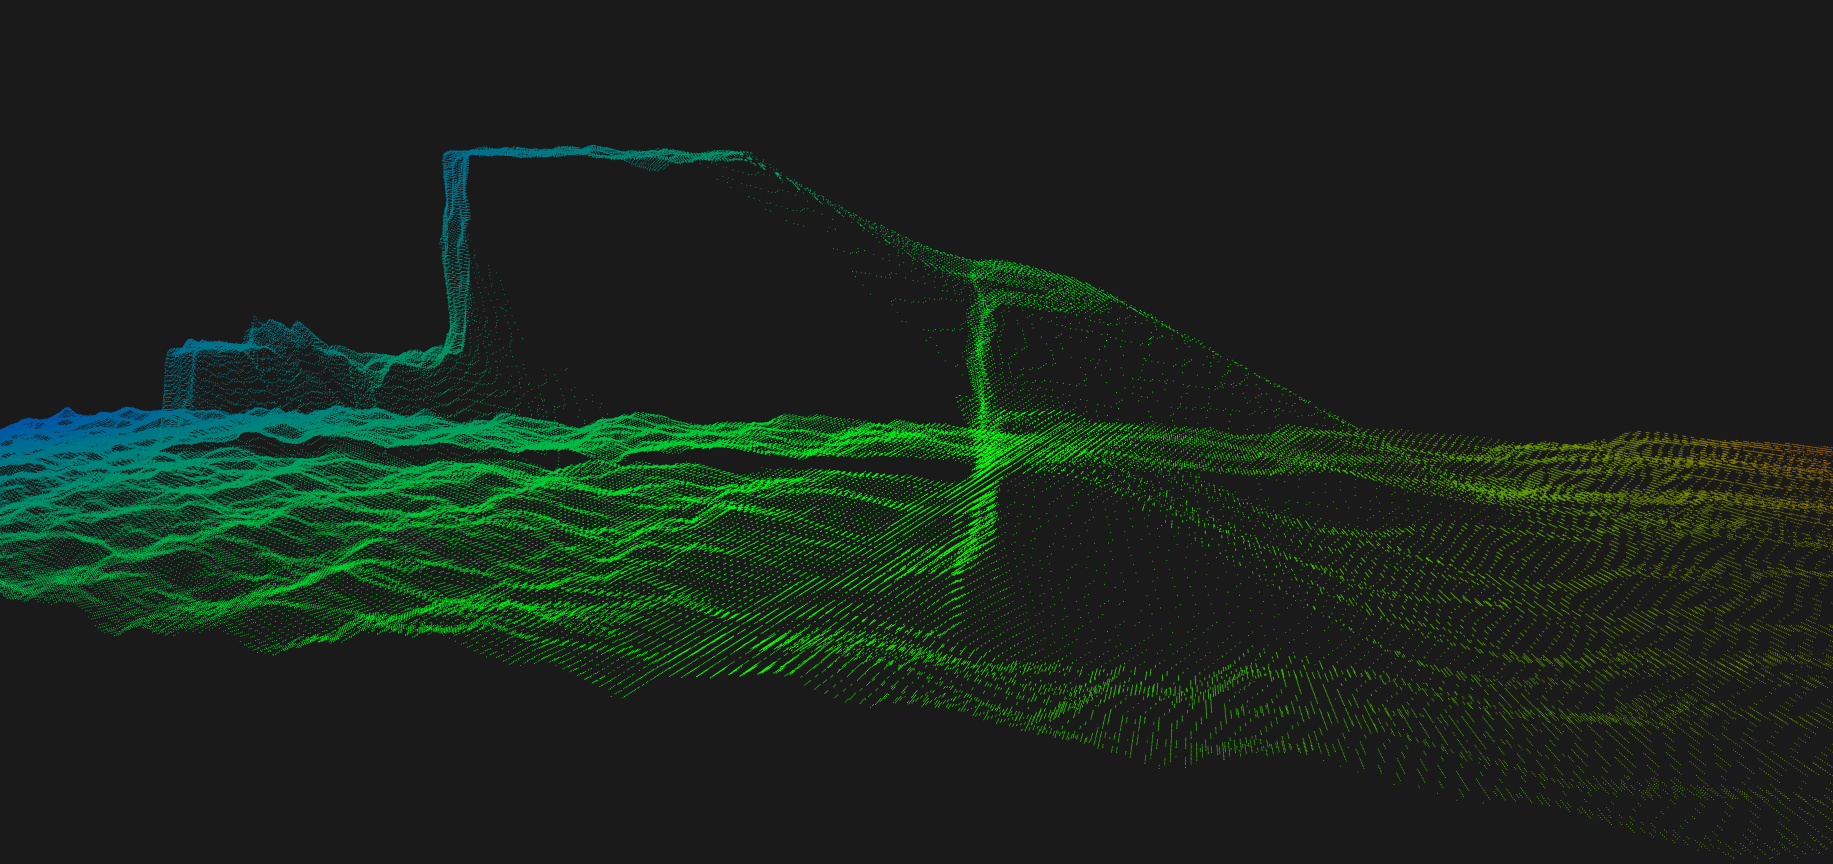
\includegraphics[width = 0.8\textwidth]{pc_crop.png}
    %\begin{wrapfigure}{r}{0.3\textwidth}
        %\centering
        %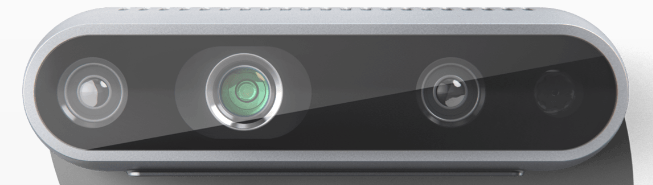
\includegraphics[width = 0.28\textwidth]{realsense_kamera.png}
    %\end{wrapfigure}
    %\begin{figure}[b]
        %\centering
        %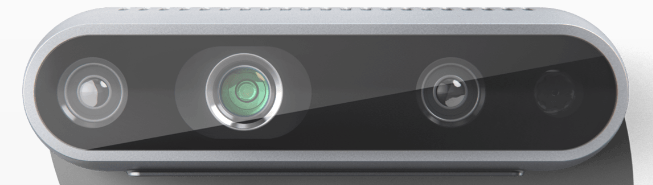
\includegraphics[width = 0.8\linewidth]{realsense_kamera.png}
    %\end{figure}
\end{frame}
%\placelogotrue
\begin{frame}
    \frametitle{Postup detekce}
    \begin{enumerate}
        \item Detekce normálového vektoru země
            \begin{itemize}
                \item Pomocí Random Sample Consensus (RANSAC) algoritmu.
                \item Určení gradientu výšky v každém bodě a následné sloučení do shluků.
                \item Postup založený na analýze hlavních komponent (PCA).
            \end{itemize}
        \item[~] 
        \item Prahování bodů podle vzdálenosti od země
        \item[~] 
        \item Detekce polohy jednotlivých cihel
            \begin{itemize}
                \item Pomocí otáčejícíh se třmenů.
                \item Pomocí RANSAC algoritmu.
            \end{itemize}
    \end{enumerate}
\end{frame}

\begin{frame}
    \frametitle{Detekce normálového vektoru země pomocí PCA}
    \begin{minipage}{0.39\textwidth}
        \begin{itemize}
            \item Statická maska 40-ti bodů
            \item Proložení pomocí PCA
            \item Expandování bodů
            \item Opětovné proložení pomocí PCA
        \end{itemize}
    \end{minipage}
    \begin{minipage}{0.60\textwidth}
    \begin{figure}
        \centering
        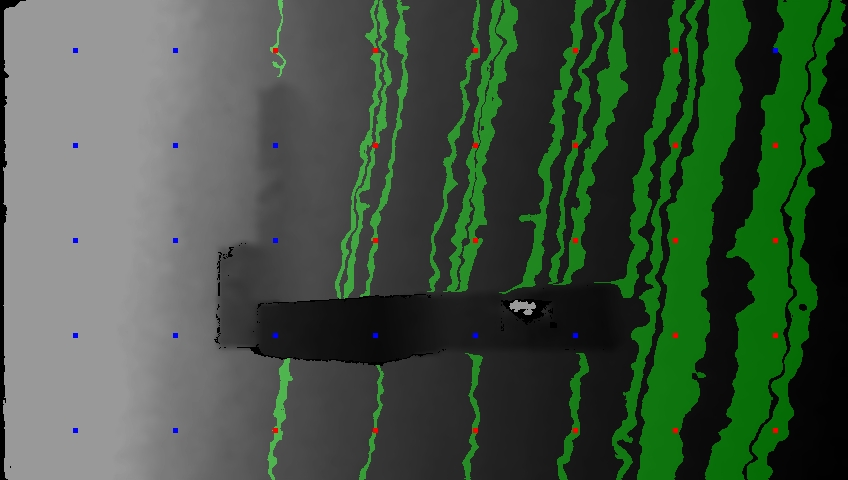
\includegraphics[width = \linewidth]{PCA_prezentace.jpg}
    \end{figure}
    \end{minipage}

    \begin{minipage}{0.60\textwidth}
        \begin{figure}
            \centering
            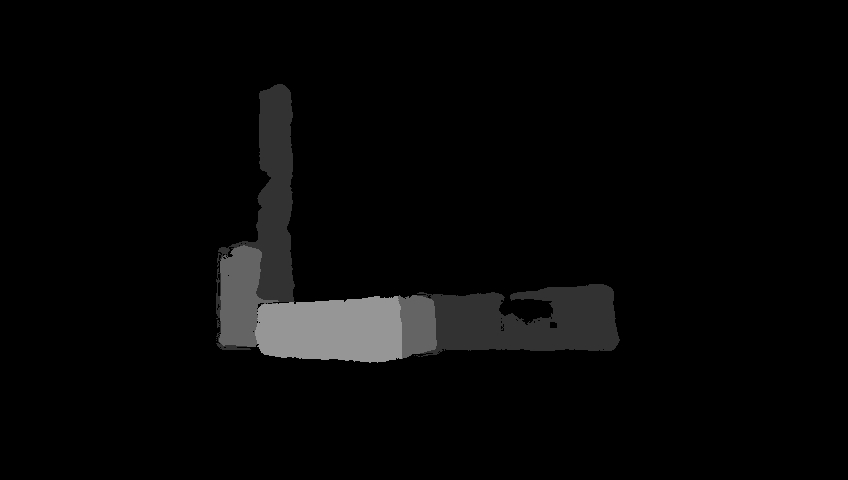
\includegraphics[width = \linewidth]{Prahovani_prezentace.jpg}
        \end{figure}
    \end{minipage}
    \begin{minipage}{0.39\textwidth}
        \begin{itemize}
            \item Určena vzdálenost bodů od země
            \item Podle vzdálenosti přiřazeno patro zdi
        \end{itemize}
    \end{minipage}
\end{frame}

%\begin{frame}
    %\frametitle{Obraz po prahování}
    %\begin{figure}
        %\centering
        %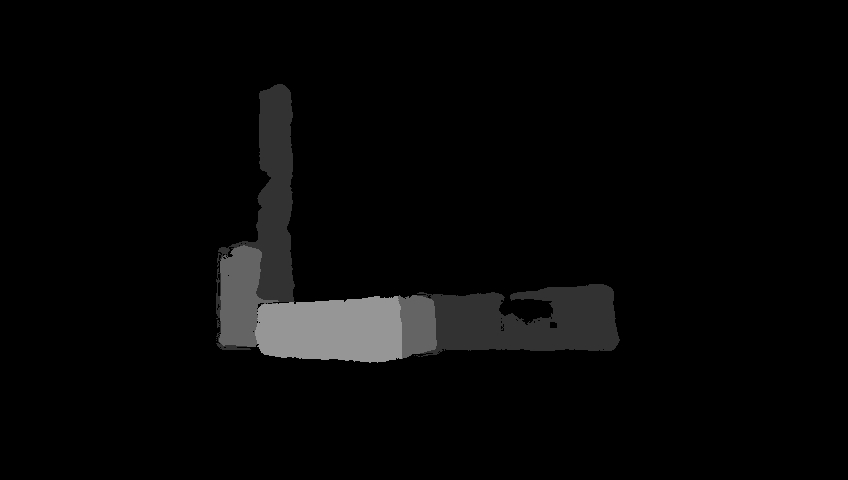
\includegraphics[width = \linewidth]{Prahovani_prezentace.jpg}
    %\end{figure}
%\end{frame}

\begin{frame}
    \frametitle{Detekce pozice cihel z prahovaných dat pomocí RANSAC}
    \begin{minipage}{0.40\textwidth}
    \begin{itemize}
        \item Detekce obrysu shluku
        \item Rotace obrysu 
        \item Nalezení přímky v obrysu
        \item Nalezení parelelní přímky
        %\item Určení polohy cihly 
            %\begin{itemize}
                %\item Otáčející třemeny
                %\item RANSAC
            %\end{itemize}
    \end{itemize}
    \end{minipage}
    \begin{minipage}{0.59\textwidth}
    \begin{figure}
        \centering
        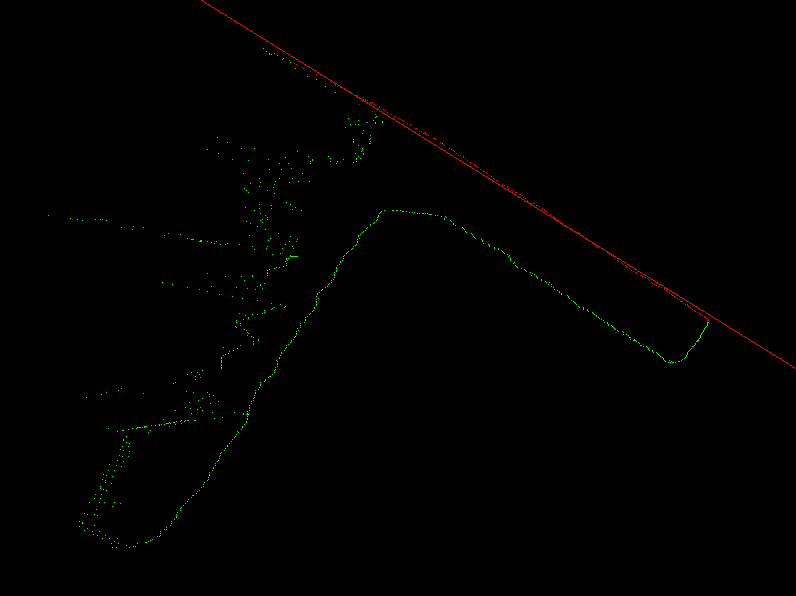
\includegraphics[width = \linewidth]{ransac_rect_fit1.png}
    \end{figure}
    \end{minipage}
    \begin{minipage}{0.59\textwidth}
        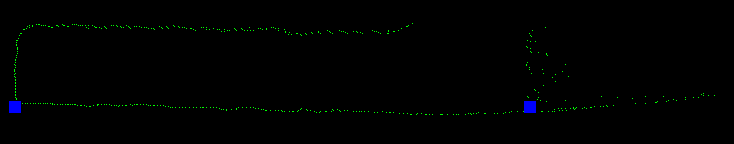
\includegraphics[width = \linewidth]{ransac_rec_fit_3_crop.png}
    \end{minipage}
    \begin{minipage}{0.40\textwidth}
    \begin{itemize}
        \item Projekce bodů mezi přímkami
        \item Nalezení maximální hustoty promítnutých bodů
    \end{itemize}
    \end{minipage}
\end{frame}

\begin{frame}
    \frametitle{Vyhodnocování výsledků}
    \begin{itemize}
        \item Pseudonáhodný výběr 20-ti a 15-ti hloubkových snímků
        \item Ručně zenesena poloha cihel
        \item Měření času běhu algoritmu na jednom jádře procesoru
    \end{itemize}
    %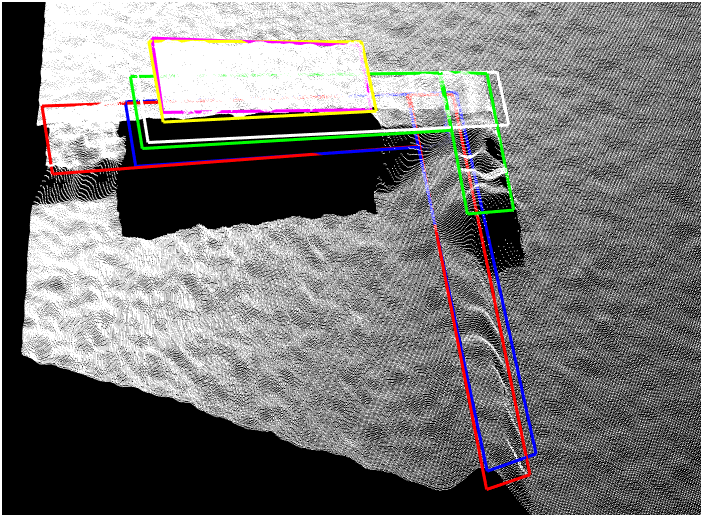
\includegraphics[width = \linewidth]{upraveno_3rdlayaer.png}
    \begin{minipage}{0.49\textwidth}
        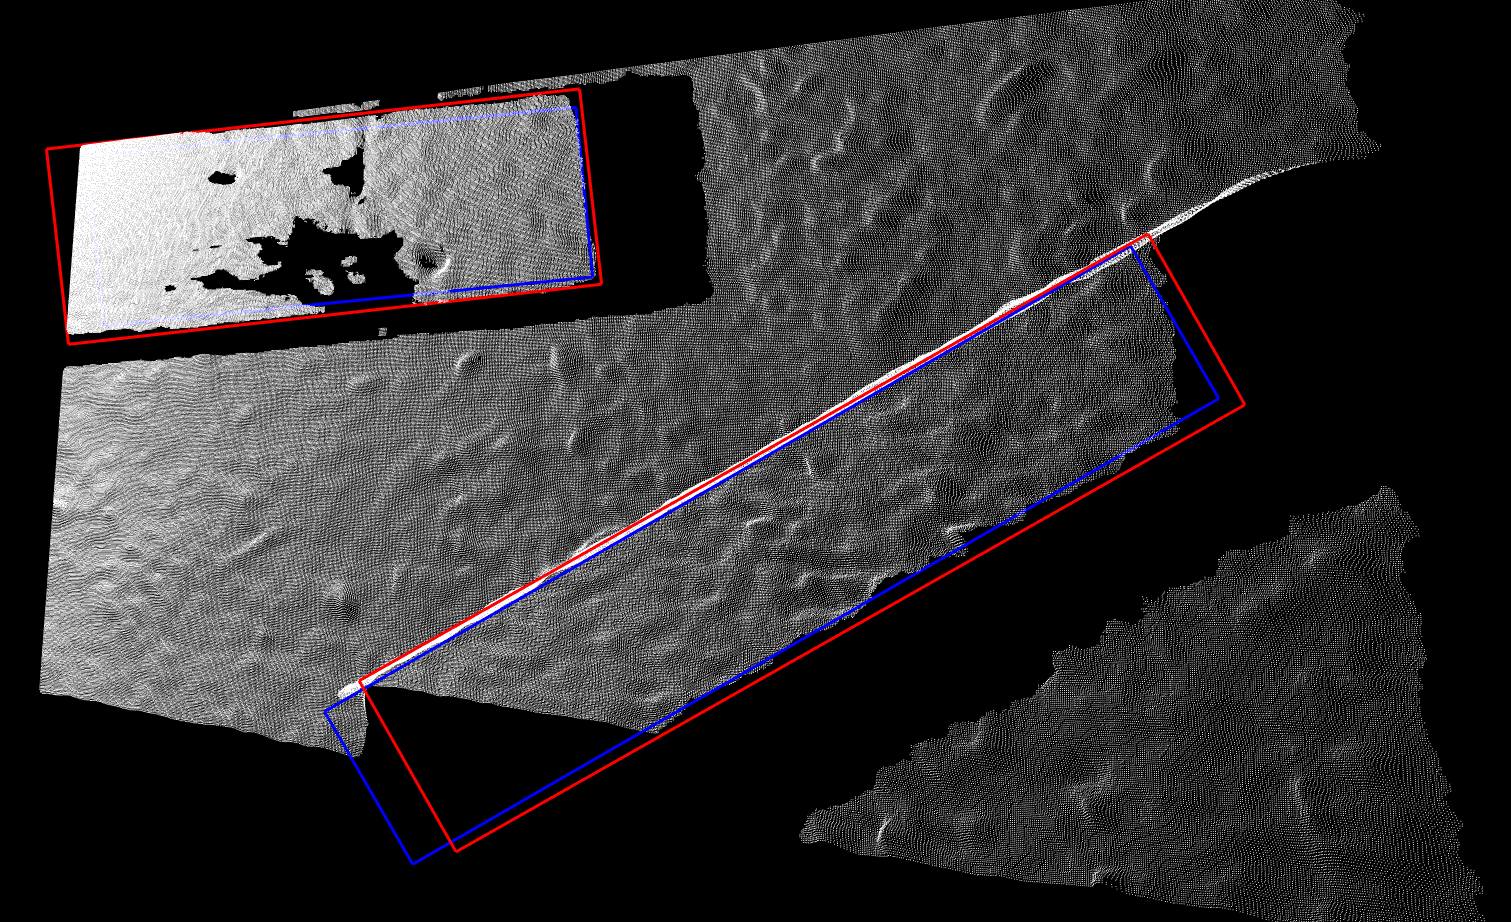
\includegraphics[width = \linewidth]{res_det_good.png}
    \end{minipage}
    \begin{minipage}{0.49\textwidth}
        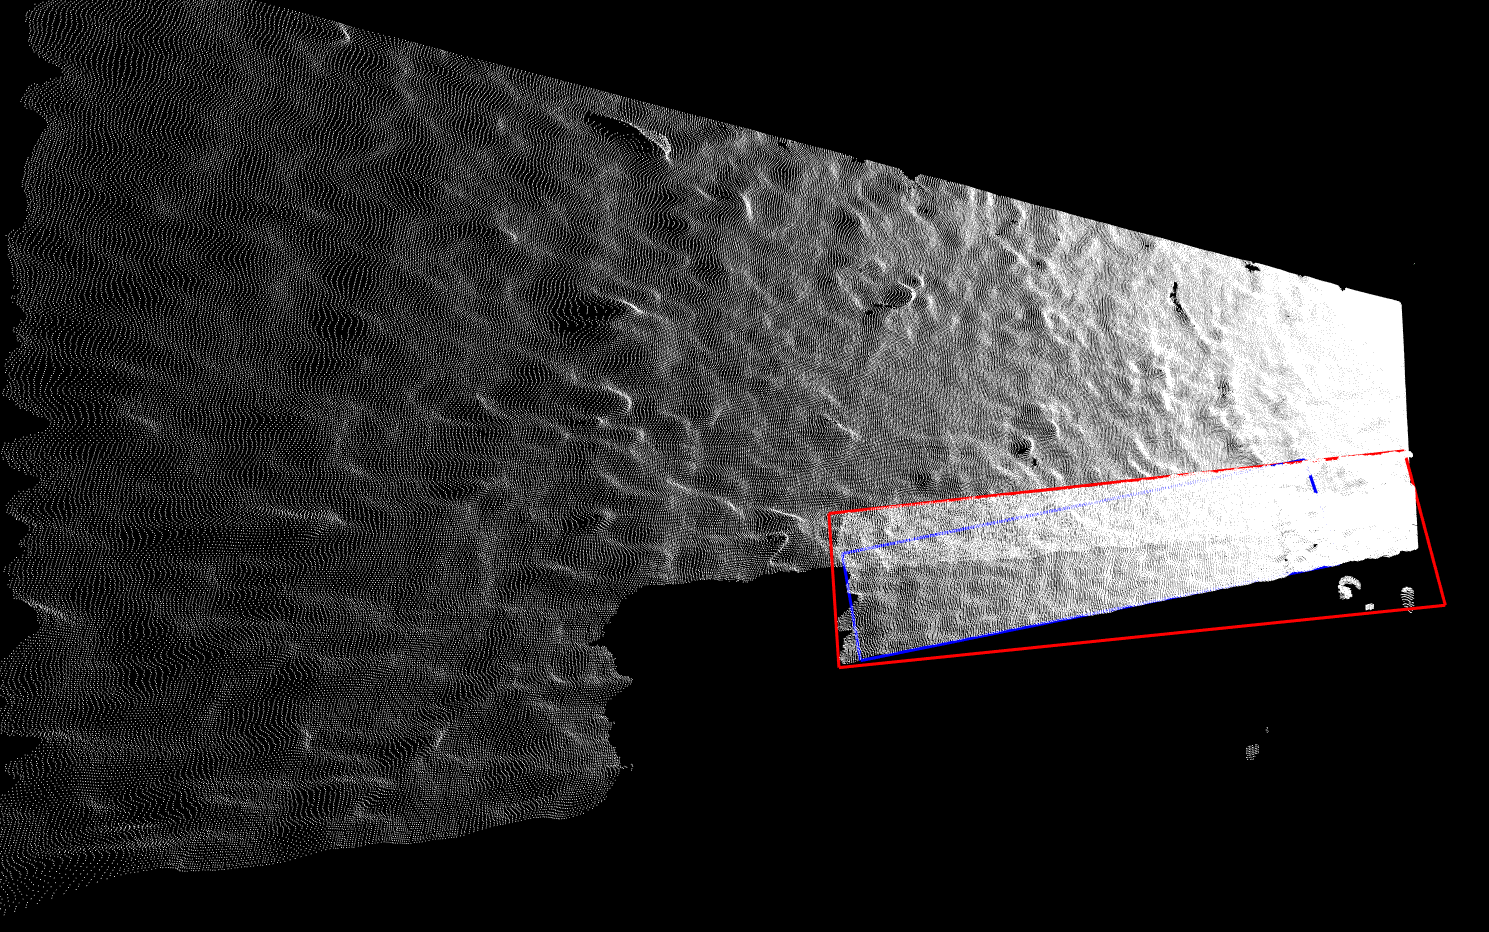
\includegraphics[width = \linewidth]{res_det_bad.png}
    \end{minipage}
\end{frame}

\begin{frame}
    \frametitle{Výsledky}
    
\begin{table}[h]
    \centering
    \begin{tabular}{|l|c|c|c|c|c|c|} \hline
        algoritmus &  přesnost [\%]& čas [ms]\\ \hline \hline
        RANSAC-$li$ a Otáčející se třmeny & 43,2 & 108 \\ \hline
        RANSAC-$hi$ a Otáčející se třmeny & 61,3 & 143 \\ \hline
        PCA-$n$ a Otáčející se třmeny & 57,5 & 148 \\ \hline 
        PCA-$v$ a Otáčející se třmeny & 65,2 & 243 \\ \hline
        RANSAC-$li$ a RANSAC-det & 58,4 & 182 \\ \hline
        \cellcolor{cvut_navy}RANSAC-$hi$ a RANSAC-det & 68,7 & 217 \\ \hline
        PCA-$n$ a RANSAC-det & 63,1 & 223 \\ \hline 
        \cellcolor{cvut_navy}PCA-$v$ a RANSAC-det & 70,8 & 328 \\ \hline
        \cellcolor{cvut_navy}PCA-$v$ a RANSAC-det - složité objekty & 68,24 & 341 \\ \hline
    \end{tabular}
    %\caption{Porovnání výsledků jednotlivých algoritmů}
    \label{tab:vysledky}
\end{table}
\end{frame}

\begin{frame}
\frametitle{Porovnání výsledků}
 %Tato práce:
 %\begin{itemize}
     %\item Přesnost detekce až 70,8\,\%
     %\item Zpracovává 5 snímků za sekundu při rozlišení 848$\times$480 pixelů 
 %\end{itemize}
 %Podobné práce: 
 \begin{itemize}
     \item \textbf{Tato práce}
         \begin{itemize}
             \item Přesnost detekce až 70,8\,\%
             \item Zpracovává 5 snímků za sekundu při rozlišení 848$\times$480 pixelů 
         \end{itemize}
    \item \textbf{Jia at al. 2013}
        \begin{itemize}
            \item Detekce objektů podobných tvarů
            \item Objetky se nachází v obecnější poloze
            \item Přesnost detekce 61,7\,\% - 70\,\%
            \item Nepracuje v reálném čase
        \end{itemize}
     \item \textbf{Holz et al. 2011} 
         \begin{itemize} 
            \item Segmentace obrazu na jednotlivé instance
            \item Přesnost segmentace 93\,\%
            \item Zpracovává 7 snímků za sekundu při rozlišení 640$\times$480 pixelů
         \end{itemize}
 \end{itemize}
\end{frame}

\begin{frame}
    \frametitle{Závěr}
    \begin{itemize}
        \item Vyzkoušeno několik metod detekce cihel
        \item Přesnost detekce až 70,8\,\%
        \item Při přesnosti nad 68\,\% pouze 5 snímků za sekundu
    \end{itemize}    
    Návrhy na zlepšení:
    \begin{itemize}
        \item Použití výkonějšího hardwaru
        \item Paralelizace programu
        \item Použití LIDARu
    \end{itemize}
\end{frame}


\begin{frame}
    \begin{center}
    \huge Děkuji za pozornost.
    \end{center}    
\end{frame}
\end{document}
